\documentclass[1p]{elsarticle_modified}
%\bibliographystyle{elsarticle-num}

%\usepackage[colorlinks]{hyperref}
%\usepackage{abbrmath_seonhwa} %\Abb, \Ascr, \Acal ,\Abf, \Afrak
\usepackage{amsfonts}
\usepackage{amssymb}
\usepackage{amsmath}
\usepackage{amsthm}
\usepackage{scalefnt}
\usepackage{amsbsy}
\usepackage{kotex}
\usepackage{caption}
\usepackage{subfig}
\usepackage{color}
\usepackage{graphicx}
\usepackage{xcolor} %% white, black, red, green, blue, cyan, magenta, yellow
\usepackage{float}
\usepackage{setspace}
\usepackage{hyperref}

\usepackage{tikz}
\usetikzlibrary{arrows}

\usepackage{multirow}
\usepackage{array} % fixed length table
\usepackage{hhline}

%%%%%%%%%%%%%%%%%%%%%
\makeatletter
\renewcommand*\env@matrix[1][\arraystretch]{%
	\edef\arraystretch{#1}%
	\hskip -\arraycolsep
	\let\@ifnextchar\new@ifnextchar
	\array{*\c@MaxMatrixCols c}}
\makeatother %https://tex.stackexchange.com/questions/14071/how-can-i-increase-the-line-spacing-in-a-matrix
%%%%%%%%%%%%%%%

\usepackage[normalem]{ulem}

\newcommand{\msout}[1]{\ifmmode\text{\sout{\ensuremath{#1}}}\else\sout{#1}\fi}
%SOURCE: \msout is \stkout macro in https://tex.stackexchange.com/questions/20609/strikeout-in-math-mode

\newcommand{\cancel}[1]{
	\ifmmode
	{\color{red}\msout{#1}}
	\else
	{\color{red}\sout{#1}}
	\fi
}

\newcommand{\add}[1]{
	{\color{blue}\uwave{#1}}
}

\newcommand{\replace}[2]{
	\ifmmode
	{\color{red}\msout{#1}}{\color{blue}\uwave{#2}}
	\else
	{\color{red}\sout{#1}}{\color{blue}\uwave{#2}}
	\fi
}

\newcommand{\Sol}{\mathcal{S}} %segment
\newcommand{\D}{D} %diagram
\newcommand{\A}{\mathcal{A}} %arc


%%%%%%%%%%%%%%%%%%%%%%%%%%%%%5 test

\def\sl{\operatorname{\textup{SL}}(2,\Cbb)}
\def\psl{\operatorname{\textup{PSL}}(2,\Cbb)}
\def\quan{\mkern 1mu \triangleright \mkern 1mu}

\theoremstyle{definition}
\newtheorem{thm}{Theorem}[section]
\newtheorem{prop}[thm]{Proposition}
\newtheorem{lem}[thm]{Lemma}
\newtheorem{ques}[thm]{Question}
\newtheorem{cor}[thm]{Corollary}
\newtheorem{defn}[thm]{Definition}
\newtheorem{exam}[thm]{Example}
\newtheorem{rmk}[thm]{Remark}
\newtheorem{alg}[thm]{Algorithm}

\newcommand{\I}{\sqrt{-1}}
\begin{document}

%\begin{frontmatter}
%
%\title{Boundary parabolic representations of knots up to 8 crossings}
%
%%% Group authors per affiliation:
%\author{Yunhi Cho} 
%\address{Department of Mathematics, University of Seoul, Seoul, Korea}
%\ead{yhcho@uos.ac.kr}
%
%
%\author{Seonhwa Kim} %\fnref{s_kim}}
%\address{Center for Geometry and Physics, Institute for Basic Science, Pohang, 37673, Korea}
%\ead{ryeona17@ibs.re.kr}
%
%\author{Hyuk Kim}
%\address{Department of Mathematical Sciences, Seoul National University, Seoul 08826, Korea}
%\ead{hyukkim@snu.ac.kr}
%
%\author{Seokbeom Yoon}
%\address{Department of Mathematical Sciences, Seoul National University, Seoul, 08826,  Korea}
%\ead{sbyoon15@snu.ac.kr}
%
%\begin{abstract}
%We find all boundary parabolic representation of knots up to 8 crossings.
%
%\end{abstract}
%\begin{keyword}
%    \MSC[2010] 57M25 
%\end{keyword}
%
%\end{frontmatter}

%\linenumbers
%\tableofcontents
%
\newcommand\colored[1]{\textcolor{white}{\rule[-0.35ex]{0.8em}{1.4ex}}\kern-0.8em\color{red} #1}%
%\newcommand\colored[1]{\textcolor{white}{ #1}\kern-2.17ex	\textcolor{white}{ #1}\kern-1.81ex	\textcolor{white}{ #1}\kern-2.15ex\color{red}#1	}

{\Large $\underline{12a_{0363}~(K12a_{0363})}$}

\setlength{\tabcolsep}{10pt}
\renewcommand{\arraystretch}{1.6}
\vspace{1cm}\begin{tabular}{m{100pt}>{\centering\arraybackslash}m{274pt}}
\multirow{5}{120pt}{
	\centering
	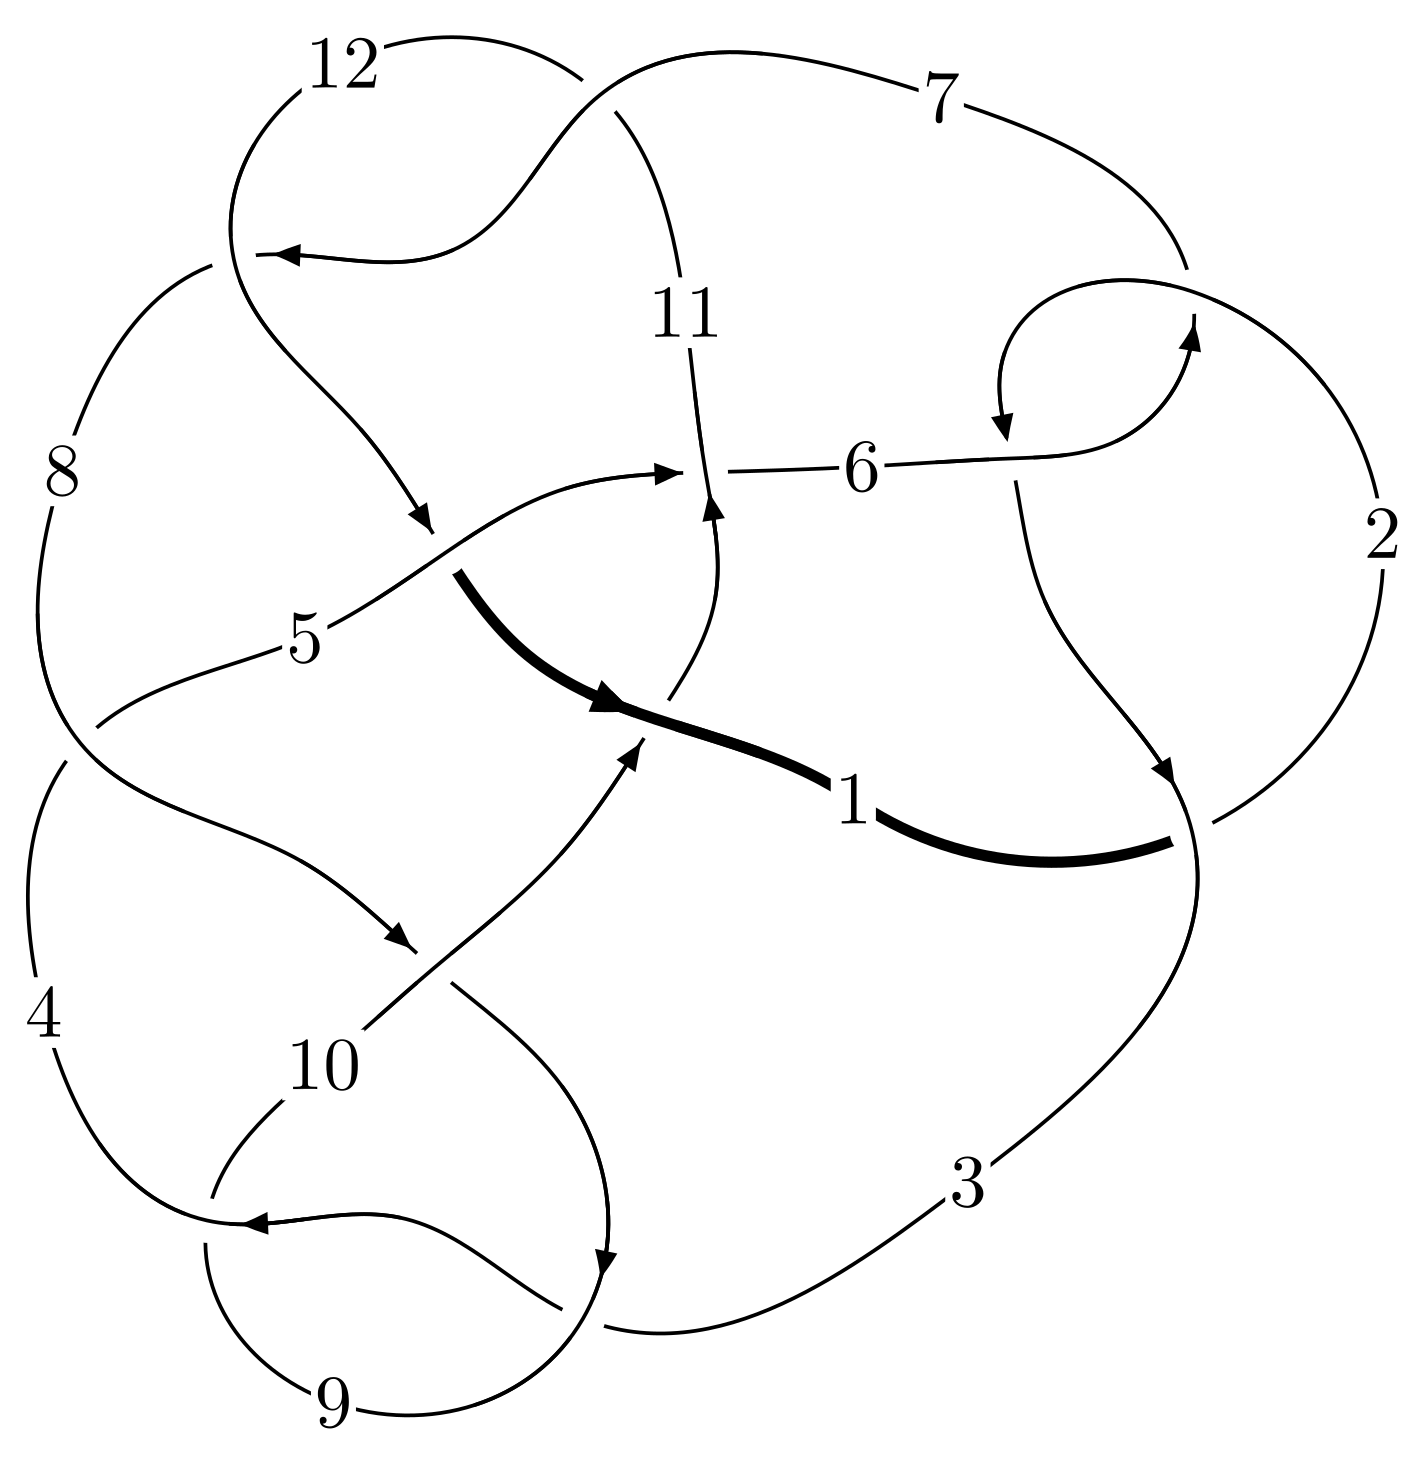
\includegraphics[width=112pt]{../../../GIT/diagram.site/Diagrams/png/1164_12a_0363.png}\\
\ \ \ A knot diagram\footnotemark}&
\allowdisplaybreaks
\textbf{Linearized knot diagam} \\
\cline{2-2}
 &
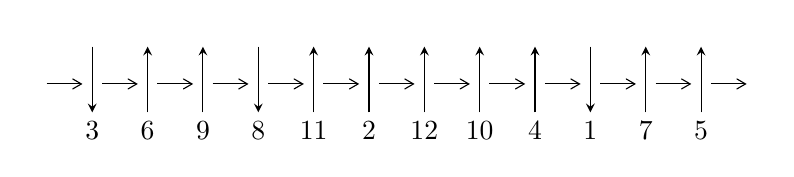
\begin{tikzpicture}[x=20pt, y=17pt]
	% nodes
	\node (C0) at (0, 0) {};
	\node (C1) at (1, 0) {};
	\node (C1U) at (1, +1) {};
	\node (C1D) at (1, -1) {3};

	\node (C2) at (2, 0) {};
	\node (C2U) at (2, +1) {};
	\node (C2D) at (2, -1) {6};

	\node (C3) at (3, 0) {};
	\node (C3U) at (3, +1) {};
	\node (C3D) at (3, -1) {9};

	\node (C4) at (4, 0) {};
	\node (C4U) at (4, +1) {};
	\node (C4D) at (4, -1) {8};

	\node (C5) at (5, 0) {};
	\node (C5U) at (5, +1) {};
	\node (C5D) at (5, -1) {11};

	\node (C6) at (6, 0) {};
	\node (C6U) at (6, +1) {};
	\node (C6D) at (6, -1) {2};

	\node (C7) at (7, 0) {};
	\node (C7U) at (7, +1) {};
	\node (C7D) at (7, -1) {12};

	\node (C8) at (8, 0) {};
	\node (C8U) at (8, +1) {};
	\node (C8D) at (8, -1) {10};

	\node (C9) at (9, 0) {};
	\node (C9U) at (9, +1) {};
	\node (C9D) at (9, -1) {4};

	\node (C10) at (10, 0) {};
	\node (C10U) at (10, +1) {};
	\node (C10D) at (10, -1) {1};

	\node (C11) at (11, 0) {};
	\node (C11U) at (11, +1) {};
	\node (C11D) at (11, -1) {7};

	\node (C12) at (12, 0) {};
	\node (C12U) at (12, +1) {};
	\node (C12D) at (12, -1) {5};
	\node (C13) at (13, 0) {};

	% arrows
	\draw[->,>={angle 60}]
	(C0) edge (C1) (C1) edge (C2) (C2) edge (C3) (C3) edge (C4) (C4) edge (C5) (C5) edge (C6) (C6) edge (C7) (C7) edge (C8) (C8) edge (C9) (C9) edge (C10) (C10) edge (C11) (C11) edge (C12) (C12) edge (C13) ;	\draw[->,>=stealth]
	(C1U) edge (C1D) (C2D) edge (C2U) (C3D) edge (C3U) (C4U) edge (C4D) (C5D) edge (C5U) (C6D) edge (C6U) (C7D) edge (C7U) (C8D) edge (C8U) (C9D) edge (C9U) (C10U) edge (C10D) (C11D) edge (C11U) (C12D) edge (C12U) ;
	\end{tikzpicture} \\
\hhline{~~} \\& 
\textbf{Solving Sequence} \\ \cline{2-2} 
 &
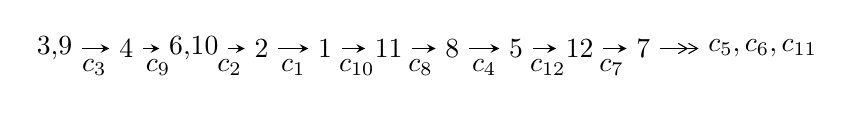
\begin{tikzpicture}[x=23pt, y=7pt]
	% node
	\node (A0) at (-1/8, 0) {3,9};
	\node (A1) at (1, 0) {4};
	\node (A2) at (33/16, 0) {6,10};
	\node (A3) at (25/8, 0) {2};
	\node (A4) at (33/8, 0) {1};
	\node (A5) at (41/8, 0) {11};
	\node (A6) at (49/8, 0) {8};
	\node (A7) at (57/8, 0) {5};
	\node (A8) at (65/8, 0) {12};
	\node (A9) at (73/8, 0) {7};
	\node (C1) at (1/2, -1) {$c_{3}$};
	\node (C2) at (3/2, -1) {$c_{9}$};
	\node (C3) at (21/8, -1) {$c_{2}$};
	\node (C4) at (29/8, -1) {$c_{1}$};
	\node (C5) at (37/8, -1) {$c_{10}$};
	\node (C6) at (45/8, -1) {$c_{8}$};
	\node (C7) at (53/8, -1) {$c_{4}$};
	\node (C8) at (61/8, -1) {$c_{12}$};
	\node (C9) at (69/8, -1) {$c_{7}$};
	\node (A10) at (11, 0) {$c_{5},c_{6},c_{11}$};

	% edge
	\draw[->,>=stealth]	
	(A0) edge (A1) (A1) edge (A2) (A2) edge (A3) (A3) edge (A4) (A4) edge (A5) (A5) edge (A6) (A6) edge (A7) (A7) edge (A8) (A8) edge (A9) ;
	\draw[->>,>={angle 60}]	
	(A9) edge (A10);
\end{tikzpicture} \\ 

\end{tabular} \\

\footnotetext{
The image of knot diagram is generated by the software ``\textbf{Draw programme}" developed by Andrew Bartholomew(\url{http://www.layer8.co.uk/maths/draw/index.htm\#Running-draw}), where we modified some parts for our purpose(\url{https://github.com/CATsTAILs/LinksPainter}).
}\phantom \\ \newline 
\centering \textbf{Ideals for irreducible components\footnotemark of $X_{\text{par}}$} 
 
\begin{align*}
I^u_{1}&=\langle 
6.13651\times10^{190} u^{139}-2.21719\times10^{190} u^{138}+\cdots+1.74140\times10^{190} b+8.78867\times10^{191},\\
\phantom{I^u_{1}}&\phantom{= \langle  }-2.57843\times10^{192} u^{139}+1.13373\times10^{192} u^{138}+\cdots+1.91554\times10^{191} a-2.84745\times10^{193},\\
\phantom{I^u_{1}}&\phantom{= \langle  }u^{140}- u^{139}+\cdots+3 u-11\rangle \\
I^u_{2}&=\langle 
-5 u^{25}+33 u^{23}+\cdots+b+1,\;10 u^{25}+8 u^{24}+\cdots+a-17,\;u^{26}-7 u^{24}+\cdots-5 u^2+1\rangle \\
\\
\end{align*}
\raggedright * 2 irreducible components of $\dim_{\mathbb{C}}=0$, with total 166 representations.\\
\footnotetext{All coefficients of polynomials are rational numbers. But the coefficients are sometimes approximated in decimal forms when there is not enough margin.}
\newpage
\renewcommand{\arraystretch}{1}
\centering \section*{I. $I^u_{1}= \langle 6.14\times10^{190} u^{139}-2.22\times10^{190} u^{138}+\cdots+1.74\times10^{190} b+8.79\times10^{191},\;-2.58\times10^{192} u^{139}+1.13\times10^{192} u^{138}+\cdots+1.92\times10^{191} a-2.85\times10^{193},\;u^{140}- u^{139}+\cdots+3 u-11 \rangle$}
\flushleft \textbf{(i) Arc colorings}\\
\begin{tabular}{m{7pt} m{180pt} m{7pt} m{180pt} }
\flushright $a_{3}=$&$\begin{pmatrix}1\\0\end{pmatrix}$ \\
\flushright $a_{9}=$&$\begin{pmatrix}0\\u\end{pmatrix}$ \\
\flushright $a_{4}=$&$\begin{pmatrix}1\\- u^2\end{pmatrix}$ \\
\flushright $a_{6}=$&$\begin{pmatrix}13.4606 u^{139}-5.91858 u^{138}+\cdots+177.633 u+148.650\\-3.52390 u^{139}+1.27322 u^{138}+\cdots-71.2813 u-50.4690\end{pmatrix}$ \\
\flushright $a_{10}=$&$\begin{pmatrix}u\\- u^3+u\end{pmatrix}$ \\
\flushright $a_{2}=$&$\begin{pmatrix}2.65083 u^{139}-3.89431 u^{138}+\cdots+111.399 u+82.2790\\3.04276 u^{139}+1.43378 u^{138}+\cdots+1.82150 u+47.9135\end{pmatrix}$ \\
\flushright $a_{1}=$&$\begin{pmatrix}5.69359 u^{139}-2.46052 u^{138}+\cdots+113.221 u+130.193\\3.04276 u^{139}+1.43378 u^{138}+\cdots+1.82150 u+47.9135\end{pmatrix}$ \\
\flushright $a_{11}=$&$\begin{pmatrix}4.08136 u^{139}-4.79781 u^{138}+\cdots+109.917 u+54.4416\\-0.606961 u^{139}+0.806119 u^{138}+\cdots-37.3582 u-6.65478\end{pmatrix}$ \\
\flushright $a_{8}=$&$\begin{pmatrix}- u^3\\u^5- u^3+u\end{pmatrix}$ \\
\flushright $a_{5}=$&$\begin{pmatrix}u^6- u^4+1\\- u^8+2 u^6-2 u^4\end{pmatrix}$ \\
\flushright $a_{12}=$&$\begin{pmatrix}3.82378 u^{139}-2.26440 u^{138}+\cdots+91.3649 u+97.7676\\3.89747 u^{139}+1.15101 u^{138}+\cdots+15.4401 u+61.6666\end{pmatrix}$ \\
\flushright $a_{7}=$&$\begin{pmatrix}4.67478 u^{139}-4.01428 u^{138}+\cdots+108.440 u+70.0227\\0.589215 u^{139}-0.565928 u^{138}+\cdots+33.8266 u+15.2231\end{pmatrix}$\\&\end{tabular}
\flushleft \textbf{(ii) Obstruction class $= -1$}\\~\\
\flushleft \textbf{(iii) Cusp Shapes $= -8.36211 u^{139}-4.62818 u^{138}+\cdots+41.7553 u-36.0403$}\\~\\
\newpage\renewcommand{\arraystretch}{1}
\flushleft \textbf{(iv) u-Polynomials at the component}\newline \\
\begin{tabular}{m{50pt}|m{274pt}}
Crossings & \hspace{64pt}u-Polynomials at each crossing \\
\hline $$\begin{aligned}c_{1}\end{aligned}$$&$\begin{aligned}
&u^{140}+52 u^{139}+\cdots+337740 u+6241
\end{aligned}$\\
\hline $$\begin{aligned}c_{2},c_{6}\end{aligned}$$&$\begin{aligned}
&u^{140}+26 u^{138}+\cdots-482 u+79
\end{aligned}$\\
\hline $$\begin{aligned}c_{3},c_{9}\end{aligned}$$&$\begin{aligned}
&u^{140}+u^{139}+\cdots-3 u-11
\end{aligned}$\\
\hline $$\begin{aligned}c_{4}\end{aligned}$$&$\begin{aligned}
&u^{140}+3 u^{139}+\cdots-25984085 u-6280527
\end{aligned}$\\
\hline $$\begin{aligned}c_{5}\end{aligned}$$&$\begin{aligned}
&u^{140}+u^{139}+\cdots+404117 u-144771
\end{aligned}$\\
\hline $$\begin{aligned}c_{7},c_{11}\end{aligned}$$&$\begin{aligned}
&u^{140}+u^{139}+\cdots+45 u-1
\end{aligned}$\\
\hline $$\begin{aligned}c_{8}\end{aligned}$$&$\begin{aligned}
&u^{140}-73 u^{139}+\cdots-1461 u+121
\end{aligned}$\\
\hline $$\begin{aligned}c_{10}\end{aligned}$$&$\begin{aligned}
&u^{140}-23 u^{139}+\cdots-258635 u+11863
\end{aligned}$\\
\hline $$\begin{aligned}c_{12}\end{aligned}$$&$\begin{aligned}
&u^{140}-3 u^{139}+\cdots-3347197 u+538957
\end{aligned}$\\
\hline
\end{tabular}\\~\\
\newpage\renewcommand{\arraystretch}{1}
\flushleft \textbf{(v) Riley Polynomials at the component}\newline \\
\begin{tabular}{m{50pt}|m{274pt}}
Crossings & \hspace{64pt}Riley Polynomials at each crossing \\
\hline $$\begin{aligned}c_{1}\end{aligned}$$&$\begin{aligned}
&y^{140}+84 y^{139}+\cdots-2917146088 y+38950081
\end{aligned}$\\
\hline $$\begin{aligned}c_{2},c_{6}\end{aligned}$$&$\begin{aligned}
&y^{140}+52 y^{139}+\cdots+337740 y+6241
\end{aligned}$\\
\hline $$\begin{aligned}c_{3},c_{9}\end{aligned}$$&$\begin{aligned}
&y^{140}-73 y^{139}+\cdots-1461 y+121
\end{aligned}$\\
\hline $$\begin{aligned}c_{4}\end{aligned}$$&$\begin{aligned}
&y^{140}+91 y^{139}+\cdots-1096216389691129 y+39445019397729
\end{aligned}$\\
\hline $$\begin{aligned}c_{5}\end{aligned}$$&$\begin{aligned}
&y^{140}-39 y^{139}+\cdots-438067087459 y+20958642441
\end{aligned}$\\
\hline $$\begin{aligned}c_{7},c_{11}\end{aligned}$$&$\begin{aligned}
&y^{140}-117 y^{139}+\cdots+107 y+1
\end{aligned}$\\
\hline $$\begin{aligned}c_{8}\end{aligned}$$&$\begin{aligned}
&y^{140}-9 y^{139}+\cdots-804005 y+14641
\end{aligned}$\\
\hline $$\begin{aligned}c_{10}\end{aligned}$$&$\begin{aligned}
&y^{140}+29 y^{139}+\cdots-922560827 y+140730769
\end{aligned}$\\
\hline $$\begin{aligned}c_{12}\end{aligned}$$&$\begin{aligned}
&y^{140}-43 y^{139}+\cdots-16999596958743 y+290474647849
\end{aligned}$\\
\hline
\end{tabular}\\~\\
\newpage\flushleft \textbf{(vi) Complex Volumes and Cusp Shapes}
$$\begin{array}{c|c|c}  
\text{Solutions to }I^u_{1}& \I (\text{vol} + \sqrt{-1}CS) & \text{Cusp shape}\\
 \hline 
\begin{aligned}
u &= -0.819465 + 0.601104 I \\
a &= -0.273785 - 0.601175 I \\
b &= -0.526903 - 0.936919 I\end{aligned}
 & -1.91446 + 1.71102 I & \phantom{-0.000000 } 0 \\ \hline\begin{aligned}
u &= -0.819465 - 0.601104 I \\
a &= -0.273785 + 0.601175 I \\
b &= -0.526903 + 0.936919 I\end{aligned}
 & -1.91446 - 1.71102 I & \phantom{-0.000000 } 0 \\ \hline\begin{aligned}
u &= \phantom{-}0.208895 + 0.998000 I \\
a &= \phantom{-}0.738442 - 0.049131 I \\
b &= -0.629531 - 0.861460 I\end{aligned}
 & \phantom{-}3.98141 + 1.29056 I & \phantom{-0.000000 } 0 \\ \hline\begin{aligned}
u &= \phantom{-}0.208895 - 0.998000 I \\
a &= \phantom{-}0.738442 + 0.049131 I \\
b &= -0.629531 + 0.861460 I\end{aligned}
 & \phantom{-}3.98141 - 1.29056 I & \phantom{-0.000000 } 0 \\ \hline\begin{aligned}
u &= \phantom{-}0.725777 + 0.641046 I \\
a &= \phantom{-}0.361709 - 0.866119 I \\
b &= \phantom{-}0.012192 - 1.196540 I\end{aligned}
 & -2.90283 + 4.25393 I & \phantom{-0.000000 } 0 \\ \hline\begin{aligned}
u &= \phantom{-}0.725777 - 0.641046 I \\
a &= \phantom{-}0.361709 + 0.866119 I \\
b &= \phantom{-}0.012192 + 1.196540 I\end{aligned}
 & -2.90283 - 4.25393 I & \phantom{-0.000000 } 0 \\ \hline\begin{aligned}
u &= -0.280451 + 0.996079 I \\
a &= \phantom{-}0.991224 - 0.455528 I \\
b &= -0.627884 - 0.845310 I\end{aligned}
 & \phantom{-}4.03314 + 3.63347 I & \phantom{-0.000000 } 0 \\ \hline\begin{aligned}
u &= -0.280451 - 0.996079 I \\
a &= \phantom{-}0.991224 + 0.455528 I \\
b &= -0.627884 + 0.845310 I\end{aligned}
 & \phantom{-}4.03314 - 3.63347 I & \phantom{-0.000000 } 0 \\ \hline\begin{aligned}
u &= \phantom{-}0.904664 + 0.324825 I \\
a &= \phantom{-}0.84139 - 1.90792 I \\
b &= -0.161953 + 0.649634 I\end{aligned}
 & -1.85564 + 1.33643 I & \phantom{-0.000000 } 0 \\ \hline\begin{aligned}
u &= \phantom{-}0.904664 - 0.324825 I \\
a &= \phantom{-}0.84139 + 1.90792 I \\
b &= -0.161953 - 0.649634 I\end{aligned}
 & -1.85564 - 1.33643 I & \phantom{-0.000000 } 0\\
 \hline 
 \end{array}$$\newpage$$\begin{array}{c|c|c}  
\text{Solutions to }I^u_{1}& \I (\text{vol} + \sqrt{-1}CS) & \text{Cusp shape}\\
 \hline 
\begin{aligned}
u &= -0.741408 + 0.605549 I \\
a &= -1.23895 - 1.65423 I \\
b &= \phantom{-}0.567177 - 0.983427 I\end{aligned}
 & -2.13460 - 6.43998 I & \phantom{-0.000000 } 0 \\ \hline\begin{aligned}
u &= -0.741408 - 0.605549 I \\
a &= -1.23895 + 1.65423 I \\
b &= \phantom{-}0.567177 + 0.983427 I\end{aligned}
 & -2.13460 + 6.43998 I & \phantom{-0.000000 } 0 \\ \hline\begin{aligned}
u &= -0.588581 + 0.752891 I \\
a &= \phantom{-}0.932767 + 0.669322 I \\
b &= -0.581080 + 0.505008 I\end{aligned}
 & \phantom{-}2.01572 + 1.08008 I & \phantom{-0.000000 } 0 \\ \hline\begin{aligned}
u &= -0.588581 - 0.752891 I \\
a &= \phantom{-}0.932767 - 0.669322 I \\
b &= -0.581080 - 0.505008 I\end{aligned}
 & \phantom{-}2.01572 - 1.08008 I & \phantom{-0.000000 } 0 \\ \hline\begin{aligned}
u &= \phantom{-}0.840582 + 0.637624 I \\
a &= \phantom{-}1.35916 - 0.66753 I \\
b &= -0.106758 - 1.116930 I\end{aligned}
 & -2.58040 + 0.68173 I & \phantom{-0.000000 } 0 \\ \hline\begin{aligned}
u &= \phantom{-}0.840582 - 0.637624 I \\
a &= \phantom{-}1.35916 + 0.66753 I \\
b &= -0.106758 + 1.116930 I\end{aligned}
 & -2.58040 - 0.68173 I & \phantom{-0.000000 } 0 \\ \hline\begin{aligned}
u &= \phantom{-}0.791527 + 0.515926 I \\
a &= \phantom{-}0.485552 + 0.133390 I \\
b &= \phantom{-}0.436044 - 0.572285 I\end{aligned}
 & -0.96654 + 2.06636 I & \phantom{-0.000000 } 0 \\ \hline\begin{aligned}
u &= \phantom{-}0.791527 - 0.515926 I \\
a &= \phantom{-}0.485552 - 0.133390 I \\
b &= \phantom{-}0.436044 + 0.572285 I\end{aligned}
 & -0.96654 - 2.06636 I & \phantom{-0.000000 } 0 \\ \hline\begin{aligned}
u &= -0.903401 + 0.251863 I \\
a &= \phantom{-}1.11305 - 1.68568 I \\
b &= \phantom{-}0.483060 + 1.013160 I\end{aligned}
 & \phantom{-}3.28601 + 2.69223 I & \phantom{-0.000000 } 0 \\ \hline\begin{aligned}
u &= -0.903401 - 0.251863 I \\
a &= \phantom{-}1.11305 + 1.68568 I \\
b &= \phantom{-}0.483060 - 1.013160 I\end{aligned}
 & \phantom{-}3.28601 - 2.69223 I & \phantom{-0.000000 } 0\\
 \hline 
 \end{array}$$\newpage$$\begin{array}{c|c|c}  
\text{Solutions to }I^u_{1}& \I (\text{vol} + \sqrt{-1}CS) & \text{Cusp shape}\\
 \hline 
\begin{aligned}
u &= -0.959593 + 0.510875 I \\
a &= \phantom{-}2.44943 + 0.92553 I \\
b &= -0.293618 + 0.965605 I\end{aligned}
 & -3.27126 - 3.56568 I & \phantom{-0.000000 } 0 \\ \hline\begin{aligned}
u &= -0.959593 - 0.510875 I \\
a &= \phantom{-}2.44943 - 0.92553 I \\
b &= -0.293618 - 0.965605 I\end{aligned}
 & -3.27126 + 3.56568 I & \phantom{-0.000000 } 0 \\ \hline\begin{aligned}
u &= \phantom{-}0.713368 + 0.820999 I \\
a &= \phantom{-}0.220508 + 0.255280 I \\
b &= -0.611825 + 1.026880 I\end{aligned}
 & \phantom{-}0.58642 - 5.94419 I & \phantom{-0.000000 } 0 \\ \hline\begin{aligned}
u &= \phantom{-}0.713368 - 0.820999 I \\
a &= \phantom{-}0.220508 - 0.255280 I \\
b &= -0.611825 - 1.026880 I\end{aligned}
 & \phantom{-}0.58642 + 5.94419 I & \phantom{-0.000000 } 0 \\ \hline\begin{aligned}
u &= \phantom{-}0.781067 + 0.463227 I \\
a &= \phantom{-}0.546918 - 0.488424 I \\
b &= -0.122889 - 0.449806 I\end{aligned}
 & -1.08917 + 1.93792 I & \phantom{-0.000000 } 0 \\ \hline\begin{aligned}
u &= \phantom{-}0.781067 - 0.463227 I \\
a &= \phantom{-}0.546918 + 0.488424 I \\
b &= -0.122889 + 0.449806 I\end{aligned}
 & -1.08917 - 1.93792 I & \phantom{-0.000000 } 0 \\ \hline\begin{aligned}
u &= \phantom{-}0.220674 + 0.880594 I \\
a &= -1.185880 - 0.572351 I \\
b &= \phantom{-}0.727382 - 1.104240 I\end{aligned}
 & \phantom{-}5.2183 - 13.9708 I & \phantom{-0.000000 } 0 \\ \hline\begin{aligned}
u &= \phantom{-}0.220674 - 0.880594 I \\
a &= -1.185880 + 0.572351 I \\
b &= \phantom{-}0.727382 + 1.104240 I\end{aligned}
 & \phantom{-}5.2183 + 13.9708 I & \phantom{-0.000000 } 0 \\ \hline\begin{aligned}
u &= -0.900493 + 0.639852 I \\
a &= -0.382863 - 0.499656 I \\
b &= \phantom{-}0.785510 + 0.473472 I\end{aligned}
 & \phantom{-}2.88856 - 6.23663 I & \phantom{-0.000000 } 0 \\ \hline\begin{aligned}
u &= -0.900493 - 0.639852 I \\
a &= -0.382863 + 0.499656 I \\
b &= \phantom{-}0.785510 - 0.473472 I\end{aligned}
 & \phantom{-}2.88856 + 6.23663 I & \phantom{-0.000000 } 0\\
 \hline 
 \end{array}$$\newpage$$\begin{array}{c|c|c}  
\text{Solutions to }I^u_{1}& \I (\text{vol} + \sqrt{-1}CS) & \text{Cusp shape}\\
 \hline 
\begin{aligned}
u &= -0.197932 + 0.854508 I \\
a &= -0.578891 + 0.278552 I \\
b &= \phantom{-}0.945512 - 0.580759 I\end{aligned}
 & \phantom{-}6.84078 + 7.84586 I & \phantom{-0.000000 } 0 \\ \hline\begin{aligned}
u &= -0.197932 - 0.854508 I \\
a &= -0.578891 - 0.278552 I \\
b &= \phantom{-}0.945512 + 0.580759 I\end{aligned}
 & \phantom{-}6.84078 - 7.84586 I & \phantom{-0.000000 } 0 \\ \hline\begin{aligned}
u &= \phantom{-}1.065320 + 0.362248 I \\
a &= -1.23718 + 1.47542 I \\
b &= -0.239406 + 0.696587 I\end{aligned}
 & \phantom{-}5.72554 + 1.31498 I & \phantom{-0.000000 } 0 \\ \hline\begin{aligned}
u &= \phantom{-}1.065320 - 0.362248 I \\
a &= -1.23718 - 1.47542 I \\
b &= -0.239406 - 0.696587 I\end{aligned}
 & \phantom{-}5.72554 - 1.31498 I & \phantom{-0.000000 } 0 \\ \hline\begin{aligned}
u &= \phantom{-}1.058820 + 0.408764 I \\
a &= \phantom{-}0.447932 - 0.024635 I \\
b &= \phantom{-}0.089918 - 1.060490 I\end{aligned}
 & -0.35657 + 1.41502 I & \phantom{-0.000000 } 0 \\ \hline\begin{aligned}
u &= \phantom{-}1.058820 - 0.408764 I \\
a &= \phantom{-}0.447932 + 0.024635 I \\
b &= \phantom{-}0.089918 + 1.060490 I\end{aligned}
 & -0.35657 - 1.41502 I & \phantom{-0.000000 } 0 \\ \hline\begin{aligned}
u &= \phantom{-}0.894142 + 0.715299 I \\
a &= -1.55420 + 0.89153 I \\
b &= \phantom{-}0.643659 + 1.070540 I\end{aligned}
 & \phantom{-}1.16619 + 11.59850 I & \phantom{-0.000000 } 0 \\ \hline\begin{aligned}
u &= \phantom{-}0.894142 - 0.715299 I \\
a &= -1.55420 - 0.89153 I \\
b &= \phantom{-}0.643659 - 1.070540 I\end{aligned}
 & \phantom{-}1.16619 - 11.59850 I & \phantom{-0.000000 } 0 \\ \hline\begin{aligned}
u &= -1.112620 + 0.299776 I \\
a &= \phantom{-}0.445941 - 1.027240 I \\
b &= \phantom{-}0.308610 + 1.222730 I\end{aligned}
 & \phantom{-}3.41072 + 2.93577 I & \phantom{-0.000000 } 0 \\ \hline\begin{aligned}
u &= -1.112620 - 0.299776 I \\
a &= \phantom{-}0.445941 + 1.027240 I \\
b &= \phantom{-}0.308610 - 1.222730 I\end{aligned}
 & \phantom{-}3.41072 - 2.93577 I & \phantom{-0.000000 } 0\\
 \hline 
 \end{array}$$\newpage$$\begin{array}{c|c|c}  
\text{Solutions to }I^u_{1}& \I (\text{vol} + \sqrt{-1}CS) & \text{Cusp shape}\\
 \hline 
\begin{aligned}
u &= \phantom{-}0.805266 + 0.256270 I \\
a &= -3.13134 - 0.38971 I \\
b &= \phantom{-}0.696447 + 0.964734 I\end{aligned}
 & \phantom{-}3.20266 + 5.85000 I & \phantom{-}10.8328 - 11.3116 I \\ \hline\begin{aligned}
u &= \phantom{-}0.805266 - 0.256270 I \\
a &= -3.13134 + 0.38971 I \\
b &= \phantom{-}0.696447 - 0.964734 I\end{aligned}
 & \phantom{-}3.20266 - 5.85000 I & \phantom{-}10.8328 + 11.3116 I \\ \hline\begin{aligned}
u &= \phantom{-}0.645976 + 0.544508 I \\
a &= \phantom{-}0.749819 - 0.949600 I \\
b &= -0.386740 - 0.877417 I\end{aligned}
 & -1.34695 + 2.10493 I & \phantom{-}6.00000 + 0. I\phantom{ +0.000000I} \\ \hline\begin{aligned}
u &= \phantom{-}0.645976 - 0.544508 I \\
a &= \phantom{-}0.749819 + 0.949600 I \\
b &= -0.386740 + 0.877417 I\end{aligned}
 & -1.34695 - 2.10493 I & \phantom{-}6.00000 + 0. I\phantom{ +0.000000I} \\ \hline\begin{aligned}
u &= -0.766449 + 0.341769 I \\
a &= \phantom{-}1.204510 - 0.117120 I \\
b &= -0.897138 + 0.663381 I\end{aligned}
 & \phantom{-}3.97663 - 2.55791 I & \phantom{-}11.57076 + 6.03390 I \\ \hline\begin{aligned}
u &= -0.766449 - 0.341769 I \\
a &= \phantom{-}1.204510 + 0.117120 I \\
b &= -0.897138 - 0.663381 I\end{aligned}
 & \phantom{-}3.97663 + 2.55791 I & \phantom{-}11.57076 - 6.03390 I \\ \hline\begin{aligned}
u &= -0.428607 + 0.720357 I \\
a &= \phantom{-}1.18236 + 0.83855 I \\
b &= -0.240114 + 0.474540 I\end{aligned}
 & \phantom{-}2.03051 + 0.98271 I & \phantom{-}6.00000 - 2.59458 I \\ \hline\begin{aligned}
u &= -0.428607 - 0.720357 I \\
a &= \phantom{-}1.18236 - 0.83855 I \\
b &= -0.240114 - 0.474540 I\end{aligned}
 & \phantom{-}2.03051 - 0.98271 I & \phantom{-}6.00000 + 2.59458 I \\ \hline\begin{aligned}
u &= \phantom{-}0.836775\phantom{ +0.000000I} \\
a &= -0.207422\phantom{ +0.000000I} \\
b &= -0.879420\phantom{ +0.000000I}\end{aligned}
 & \phantom{-}5.63574\phantom{ +0.000000I} & \phantom{-}19.3000\phantom{ +0.000000I} \\ \hline\begin{aligned}
u &= -1.123800 + 0.305845 I \\
a &= -1.09854 - 1.18868 I \\
b &= \phantom{-}0.716453 + 0.948727 I\end{aligned}
 & \phantom{-}4.40051 + 0.60498 I & \phantom{-0.000000 } 0\\
 \hline 
 \end{array}$$\newpage$$\begin{array}{c|c|c}  
\text{Solutions to }I^u_{1}& \I (\text{vol} + \sqrt{-1}CS) & \text{Cusp shape}\\
 \hline 
\begin{aligned}
u &= -1.123800 - 0.305845 I \\
a &= -1.09854 + 1.18868 I \\
b &= \phantom{-}0.716453 - 0.948727 I\end{aligned}
 & \phantom{-}4.40051 - 0.60498 I & \phantom{-0.000000 } 0 \\ \hline\begin{aligned}
u &= \phantom{-}1.149630 + 0.330362 I \\
a &= \phantom{-}1.60976 - 0.69797 I \\
b &= -0.673469 + 1.009790 I\end{aligned}
 & \phantom{-}4.26218 - 4.49247 I & \phantom{-0.000000 } 0 \\ \hline\begin{aligned}
u &= \phantom{-}1.149630 - 0.330362 I \\
a &= \phantom{-}1.60976 + 0.69797 I \\
b &= -0.673469 - 1.009790 I\end{aligned}
 & \phantom{-}4.26218 + 4.49247 I & \phantom{-0.000000 } 0 \\ \hline\begin{aligned}
u &= \phantom{-}0.112882 + 0.792728 I \\
a &= \phantom{-}0.557215 + 0.068936 I \\
b &= -0.067761 + 0.609858 I\end{aligned}
 & \phantom{-}1.52861 - 1.68586 I & \phantom{-}4.68797 + 3.45114 I \\ \hline\begin{aligned}
u &= \phantom{-}0.112882 - 0.792728 I \\
a &= \phantom{-}0.557215 - 0.068936 I \\
b &= -0.067761 - 0.609858 I\end{aligned}
 & \phantom{-}1.52861 + 1.68586 I & \phantom{-}4.68797 - 3.45114 I \\ \hline\begin{aligned}
u &= \phantom{-}0.263276 + 0.754577 I \\
a &= \phantom{-}0.176137 + 0.788252 I \\
b &= -0.167287 + 1.295340 I\end{aligned}
 & -0.76781 - 5.99748 I & \phantom{-}3.63087 + 7.05574 I \\ \hline\begin{aligned}
u &= \phantom{-}0.263276 - 0.754577 I \\
a &= \phantom{-}0.176137 - 0.788252 I \\
b &= -0.167287 - 1.295340 I\end{aligned}
 & -0.76781 + 5.99748 I & \phantom{-}3.63087 - 7.05574 I \\ \hline\begin{aligned}
u &= \phantom{-}0.280187 + 0.746806 I \\
a &= \phantom{-}0.788485 + 0.671446 I \\
b &= -0.594752 + 1.020860 I\end{aligned}
 & \phantom{-}0.24157 - 3.64223 I & \phantom{-}4.72165 + 0.97424 I \\ \hline\begin{aligned}
u &= \phantom{-}0.280187 - 0.746806 I \\
a &= \phantom{-}0.788485 - 0.671446 I \\
b &= -0.594752 - 1.020860 I\end{aligned}
 & \phantom{-}0.24157 + 3.64223 I & \phantom{-}4.72165 - 0.97424 I \\ \hline\begin{aligned}
u &= -0.750280 + 0.268239 I \\
a &= -1.14819 - 2.22811 I \\
b &= \phantom{-}0.746169 + 0.729878 I\end{aligned}
 & \phantom{-}3.91151 - 0.35414 I & \phantom{-}10.25180 + 4.64821 I\\
 \hline 
 \end{array}$$\newpage$$\begin{array}{c|c|c}  
\text{Solutions to }I^u_{1}& \I (\text{vol} + \sqrt{-1}CS) & \text{Cusp shape}\\
 \hline 
\begin{aligned}
u &= -0.750280 - 0.268239 I \\
a &= -1.14819 + 2.22811 I \\
b &= \phantom{-}0.746169 - 0.729878 I\end{aligned}
 & \phantom{-}3.91151 + 0.35414 I & \phantom{-}10.25180 - 4.64821 I \\ \hline\begin{aligned}
u &= -0.229412 + 0.756603 I \\
a &= -1.35042 + 1.16217 I \\
b &= \phantom{-}0.637868 + 1.026790 I\end{aligned}
 & \phantom{-}0.17383 + 7.83476 I & \phantom{-}5.17246 - 7.94900 I \\ \hline\begin{aligned}
u &= -0.229412 - 0.756603 I \\
a &= -1.35042 - 1.16217 I \\
b &= \phantom{-}0.637868 - 1.026790 I\end{aligned}
 & \phantom{-}0.17383 - 7.83476 I & \phantom{-}5.17246 + 7.94900 I \\ \hline\begin{aligned}
u &= -1.160530 + 0.363731 I \\
a &= \phantom{-}1.53233 - 0.71195 I \\
b &= -0.739607 + 0.623924 I\end{aligned}
 & \phantom{-}5.39201 - 0.90370 I & \phantom{-0.000000 } 0 \\ \hline\begin{aligned}
u &= -1.160530 - 0.363731 I \\
a &= \phantom{-}1.53233 + 0.71195 I \\
b &= -0.739607 - 0.623924 I\end{aligned}
 & \phantom{-}5.39201 + 0.90370 I & \phantom{-0.000000 } 0 \\ \hline\begin{aligned}
u &= -1.111320 + 0.495860 I \\
a &= -1.258030 - 0.397388 I \\
b &= -0.031319 - 1.141470 I\end{aligned}
 & -1.06553 - 5.82110 I & \phantom{-0.000000 } 0 \\ \hline\begin{aligned}
u &= -1.111320 - 0.495860 I \\
a &= -1.258030 + 0.397388 I \\
b &= -0.031319 + 1.141470 I\end{aligned}
 & -1.06553 + 5.82110 I & \phantom{-0.000000 } 0 \\ \hline\begin{aligned}
u &= \phantom{-}1.164220 + 0.393081 I \\
a &= -1.81411 - 0.11891 I \\
b &= \phantom{-}0.768058 + 0.682952 I\end{aligned}
 & \phantom{-}5.17383 + 5.00452 I & \phantom{-0.000000 } 0 \\ \hline\begin{aligned}
u &= \phantom{-}1.164220 - 0.393081 I \\
a &= -1.81411 + 0.11891 I \\
b &= \phantom{-}0.768058 - 0.682952 I\end{aligned}
 & \phantom{-}5.17383 - 5.00452 I & \phantom{-0.000000 } 0 \\ \hline\begin{aligned}
u &= \phantom{-}0.748592 + 0.181734 I \\
a &= \phantom{-}0.878651 - 0.642024 I \\
b &= -0.779626 + 1.003540 I\end{aligned}
 & \phantom{-}2.97274 - 3.60491 I & \phantom{-}10.36671 + 1.22859 I\\
 \hline 
 \end{array}$$\newpage$$\begin{array}{c|c|c}  
\text{Solutions to }I^u_{1}& \I (\text{vol} + \sqrt{-1}CS) & \text{Cusp shape}\\
 \hline 
\begin{aligned}
u &= \phantom{-}0.748592 - 0.181734 I \\
a &= \phantom{-}0.878651 + 0.642024 I \\
b &= -0.779626 - 1.003540 I\end{aligned}
 & \phantom{-}2.97274 + 3.60491 I & \phantom{-}10.36671 - 1.22859 I \\ \hline\begin{aligned}
u &= \phantom{-}1.157840 + 0.417927 I \\
a &= -1.32716 + 1.59285 I \\
b &= \phantom{-}1.185410 - 0.389801 I\end{aligned}
 & \phantom{-}9.09011 + 1.84231 I & \phantom{-0.000000 } 0 \\ \hline\begin{aligned}
u &= \phantom{-}1.157840 - 0.417927 I \\
a &= -1.32716 - 1.59285 I \\
b &= \phantom{-}1.185410 + 0.389801 I\end{aligned}
 & \phantom{-}9.09011 - 1.84231 I & \phantom{-0.000000 } 0 \\ \hline\begin{aligned}
u &= \phantom{-}1.150750 + 0.437661 I \\
a &= -0.85517 + 1.59029 I \\
b &= \phantom{-}0.86610 - 1.15636 I\end{aligned}
 & \phantom{-}6.79845 - 0.84188 I & \phantom{-0.000000 } 0 \\ \hline\begin{aligned}
u &= \phantom{-}1.150750 - 0.437661 I \\
a &= -0.85517 - 1.59029 I \\
b &= \phantom{-}0.86610 + 1.15636 I\end{aligned}
 & \phantom{-}6.79845 + 0.84188 I & \phantom{-0.000000 } 0 \\ \hline\begin{aligned}
u &= -0.572554 + 0.509279 I \\
a &= -0.61241 + 1.78069 I \\
b &= \phantom{-}0.190353 + 1.009410 I\end{aligned}
 & -4.40135 - 0.63333 I & -1.24969 - 1.21453 I \\ \hline\begin{aligned}
u &= -0.572554 - 0.509279 I \\
a &= -0.61241 - 1.78069 I \\
b &= \phantom{-}0.190353 - 1.009410 I\end{aligned}
 & -4.40135 + 0.63333 I & -1.24969 + 1.21453 I \\ \hline\begin{aligned}
u &= \phantom{-}1.149570 + 0.451749 I \\
a &= \phantom{-}3.62115 - 0.51783 I \\
b &= -0.636854 - 0.872531 I\end{aligned}
 & \phantom{-}7.99476 + 4.59039 I & \phantom{-0.000000 } 0 \\ \hline\begin{aligned}
u &= \phantom{-}1.149570 - 0.451749 I \\
a &= \phantom{-}3.62115 + 0.51783 I \\
b &= -0.636854 + 0.872531 I\end{aligned}
 & \phantom{-}7.99476 - 4.59039 I & \phantom{-0.000000 } 0 \\ \hline\begin{aligned}
u &= -1.151660 + 0.448221 I \\
a &= \phantom{-}2.03999 + 1.35586 I \\
b &= -0.697290 - 0.849589 I\end{aligned}
 & \phantom{-}8.01842 - 3.49746 I & \phantom{-0.000000 } 0\\
 \hline 
 \end{array}$$\newpage$$\begin{array}{c|c|c}  
\text{Solutions to }I^u_{1}& \I (\text{vol} + \sqrt{-1}CS) & \text{Cusp shape}\\
 \hline 
\begin{aligned}
u &= -1.151660 - 0.448221 I \\
a &= \phantom{-}2.03999 - 1.35586 I \\
b &= -0.697290 + 0.849589 I\end{aligned}
 & \phantom{-}8.01842 + 3.49746 I & \phantom{-0.000000 } 0 \\ \hline\begin{aligned}
u &= \phantom{-}0.177381 + 0.742334 I \\
a &= -0.071572 - 0.448830 I \\
b &= \phantom{-}0.690228 + 0.563342 I\end{aligned}
 & \phantom{-}1.51325 - 2.67968 I & \phantom{-}7.37592 + 3.47726 I \\ \hline\begin{aligned}
u &= \phantom{-}0.177381 - 0.742334 I \\
a &= -0.071572 + 0.448830 I \\
b &= \phantom{-}0.690228 - 0.563342 I\end{aligned}
 & \phantom{-}1.51325 + 2.67968 I & \phantom{-}7.37592 - 3.47726 I \\ \hline\begin{aligned}
u &= -1.151040 + 0.461160 I \\
a &= -2.84467 - 0.14834 I \\
b &= \phantom{-}0.82302 - 1.21891 I\end{aligned}
 & \phantom{-}6.62997 - 8.93464 I & \phantom{-0.000000 } 0 \\ \hline\begin{aligned}
u &= -1.151040 - 0.461160 I \\
a &= -2.84467 + 0.14834 I \\
b &= \phantom{-}0.82302 + 1.21891 I\end{aligned}
 & \phantom{-}6.62997 + 8.93464 I & \phantom{-0.000000 } 0 \\ \hline\begin{aligned}
u &= -1.121350 + 0.557992 I \\
a &= -0.201215 + 0.594207 I \\
b &= \phantom{-}0.111316 + 0.716162 I\end{aligned}
 & \phantom{-}4.18372 - 5.94348 I & \phantom{-0.000000 } 0 \\ \hline\begin{aligned}
u &= -1.121350 - 0.557992 I \\
a &= -0.201215 - 0.594207 I \\
b &= \phantom{-}0.111316 - 0.716162 I\end{aligned}
 & \phantom{-}4.18372 + 5.94348 I & \phantom{-0.000000 } 0 \\ \hline\begin{aligned}
u &= -1.159140 + 0.475194 I \\
a &= -2.12166 - 0.42257 I \\
b &= \phantom{-}1.181410 - 0.526785 I\end{aligned}
 & \phantom{-}8.68313 - 6.36401 I & \phantom{-0.000000 } 0 \\ \hline\begin{aligned}
u &= -1.159140 - 0.475194 I \\
a &= -2.12166 + 0.42257 I \\
b &= \phantom{-}1.181410 + 0.526785 I\end{aligned}
 & \phantom{-}8.68313 + 6.36401 I & \phantom{-0.000000 } 0 \\ \hline\begin{aligned}
u &= -0.689219 + 0.285983 I \\
a &= \phantom{-}0.82099 + 1.64476 I \\
b &= -0.646260 + 1.169410 I\end{aligned}
 & \phantom{-}2.53323 - 5.41442 I & \phantom{-}5.96568 + 11.95972 I\\
 \hline 
 \end{array}$$\newpage$$\begin{array}{c|c|c}  
\text{Solutions to }I^u_{1}& \I (\text{vol} + \sqrt{-1}CS) & \text{Cusp shape}\\
 \hline 
\begin{aligned}
u &= -0.689219 - 0.285983 I \\
a &= \phantom{-}0.82099 - 1.64476 I \\
b &= -0.646260 - 1.169410 I\end{aligned}
 & \phantom{-}2.53323 + 5.41442 I & \phantom{-}5.96568 - 11.95972 I \\ \hline\begin{aligned}
u &= -1.175170 + 0.439114 I \\
a &= \phantom{-}0.66966 + 2.43954 I \\
b &= -0.642836 - 0.837836 I\end{aligned}
 & \phantom{-}8.10380 + 0.40309 I & \phantom{-0.000000 } 0 \\ \hline\begin{aligned}
u &= -1.175170 - 0.439114 I \\
a &= \phantom{-}0.66966 - 2.43954 I \\
b &= -0.642836 + 0.837836 I\end{aligned}
 & \phantom{-}8.10380 - 0.40309 I & \phantom{-0.000000 } 0 \\ \hline\begin{aligned}
u &= -1.158520 + 0.481809 I \\
a &= -0.768217 - 1.063910 I \\
b &= \phantom{-}0.744387 + 0.464103 I\end{aligned}
 & \phantom{-}4.56933 - 3.26362 I & \phantom{-0.000000 } 0 \\ \hline\begin{aligned}
u &= -1.158520 - 0.481809 I \\
a &= -0.768217 + 1.063910 I \\
b &= \phantom{-}0.744387 - 0.464103 I\end{aligned}
 & \phantom{-}4.56933 + 3.26362 I & \phantom{-0.000000 } 0 \\ \hline\begin{aligned}
u &= \phantom{-}1.172110 + 0.458685 I \\
a &= \phantom{-}2.49739 + 1.15826 I \\
b &= -0.688342 - 0.866363 I\end{aligned}
 & \phantom{-}7.96453 + 8.82066 I & \phantom{-0.000000 } 0 \\ \hline\begin{aligned}
u &= \phantom{-}1.172110 - 0.458685 I \\
a &= \phantom{-}2.49739 - 1.15826 I \\
b &= -0.688342 + 0.866363 I\end{aligned}
 & \phantom{-}7.96453 - 8.82066 I & \phantom{-0.000000 } 0 \\ \hline\begin{aligned}
u &= -1.206400 + 0.381025 I \\
a &= -0.055606 - 0.766674 I \\
b &= -0.044579 + 0.675540 I\end{aligned}
 & \phantom{-}5.49976 - 2.33349 I & \phantom{-0.000000 } 0 \\ \hline\begin{aligned}
u &= -1.206400 - 0.381025 I \\
a &= -0.055606 + 0.766674 I \\
b &= -0.044579 - 0.675540 I\end{aligned}
 & \phantom{-}5.49976 + 2.33349 I & \phantom{-0.000000 } 0 \\ \hline\begin{aligned}
u &= -0.087509 + 0.729576 I \\
a &= \phantom{-}0.481488 + 0.083455 I \\
b &= -0.609447 + 0.579754 I\end{aligned}
 & \phantom{-}1.53007 - 1.15987 I & \phantom{-}7.43225 + 3.70763 I\\
 \hline 
 \end{array}$$\newpage$$\begin{array}{c|c|c}  
\text{Solutions to }I^u_{1}& \I (\text{vol} + \sqrt{-1}CS) & \text{Cusp shape}\\
 \hline 
\begin{aligned}
u &= -0.087509 - 0.729576 I \\
a &= \phantom{-}0.481488 - 0.083455 I \\
b &= -0.609447 - 0.579754 I\end{aligned}
 & \phantom{-}1.53007 + 1.15987 I & \phantom{-}7.43225 - 3.70763 I \\ \hline\begin{aligned}
u &= \phantom{-}1.146500 + 0.537372 I \\
a &= -1.61922 - 0.09495 I \\
b &= \phantom{-}0.194322 + 1.356190 I\end{aligned}
 & \phantom{-}1.82460 + 10.85730 I & \phantom{-0.000000 } 0 \\ \hline\begin{aligned}
u &= \phantom{-}1.146500 - 0.537372 I \\
a &= -1.61922 + 0.09495 I \\
b &= \phantom{-}0.194322 - 1.356190 I\end{aligned}
 & \phantom{-}1.82460 - 10.85730 I & \phantom{-0.000000 } 0 \\ \hline\begin{aligned}
u &= \phantom{-}1.143940 + 0.543522 I \\
a &= -2.29631 + 0.37953 I \\
b &= \phantom{-}0.634804 + 1.084940 I\end{aligned}
 & \phantom{-}2.77562 + 8.52497 I & \phantom{-0.000000 } 0 \\ \hline\begin{aligned}
u &= \phantom{-}1.143940 - 0.543522 I \\
a &= -2.29631 - 0.37953 I \\
b &= \phantom{-}0.634804 - 1.084940 I\end{aligned}
 & \phantom{-}2.77562 - 8.52497 I & \phantom{-0.000000 } 0 \\ \hline\begin{aligned}
u &= \phantom{-}1.163270 + 0.510441 I \\
a &= \phantom{-}0.29398 - 1.49105 I \\
b &= -0.734529 + 0.532186 I\end{aligned}
 & \phantom{-}4.37382 + 7.36822 I & \phantom{-0.000000 } 0 \\ \hline\begin{aligned}
u &= \phantom{-}1.163270 - 0.510441 I \\
a &= \phantom{-}0.29398 + 1.49105 I \\
b &= -0.734529 - 0.532186 I\end{aligned}
 & \phantom{-}4.37382 - 7.36822 I & \phantom{-0.000000 } 0 \\ \hline\begin{aligned}
u &= -1.156860 + 0.529818 I \\
a &= \phantom{-}2.77811 + 0.81836 I \\
b &= -0.647927 + 1.047350 I\end{aligned}
 & \phantom{-}2.88783 - 12.66090 I & \phantom{-0.000000 } 0 \\ \hline\begin{aligned}
u &= -1.156860 - 0.529818 I \\
a &= \phantom{-}2.77811 - 0.81836 I \\
b &= -0.647927 - 1.047350 I\end{aligned}
 & \phantom{-}2.88783 + 12.66090 I & \phantom{-0.000000 } 0 \\ \hline\begin{aligned}
u &= \phantom{-}1.244700 + 0.323559 I \\
a &= \phantom{-}2.00246 + 0.40466 I \\
b &= -0.927208 - 0.629923 I\end{aligned}
 & \phantom{-}11.38690 - 3.94355 I & \phantom{-0.000000 } 0\\
 \hline 
 \end{array}$$\newpage$$\begin{array}{c|c|c}  
\text{Solutions to }I^u_{1}& \I (\text{vol} + \sqrt{-1}CS) & \text{Cusp shape}\\
 \hline 
\begin{aligned}
u &= \phantom{-}1.244700 - 0.323559 I \\
a &= \phantom{-}2.00246 - 0.40466 I \\
b &= -0.927208 + 0.629923 I\end{aligned}
 & \phantom{-}11.38690 + 3.94355 I & \phantom{-0.000000 } 0 \\ \hline\begin{aligned}
u &= \phantom{-}0.023047 + 0.710804 I \\
a &= -1.05257 + 1.27195 I \\
b &= \phantom{-}0.654278 - 0.878099 I\end{aligned}
 & \phantom{-}4.72416 - 4.54539 I & \phantom{-}11.00938 + 6.82756 I \\ \hline\begin{aligned}
u &= \phantom{-}0.023047 - 0.710804 I \\
a &= -1.05257 - 1.27195 I \\
b &= \phantom{-}0.654278 + 0.878099 I\end{aligned}
 & \phantom{-}4.72416 + 4.54539 I & \phantom{-}11.00938 - 6.82756 I \\ \hline\begin{aligned}
u &= \phantom{-}1.188310 + 0.501202 I \\
a &= -0.936338 - 0.411125 I \\
b &= \phantom{-}0.010051 + 0.549485 I\end{aligned}
 & \phantom{-}4.67098 + 6.41520 I & \phantom{-0.000000 } 0 \\ \hline\begin{aligned}
u &= \phantom{-}1.188310 - 0.501202 I \\
a &= -0.936338 + 0.411125 I \\
b &= \phantom{-}0.010051 - 0.549485 I\end{aligned}
 & \phantom{-}4.67098 - 6.41520 I & \phantom{-0.000000 } 0 \\ \hline\begin{aligned}
u &= -1.263960 + 0.301245 I \\
a &= \phantom{-}1.44206 + 1.06783 I \\
b &= -0.739648 - 1.076720 I\end{aligned}
 & \phantom{-}9.9965 + 10.0671 I & \phantom{-0.000000 } 0 \\ \hline\begin{aligned}
u &= -1.263960 - 0.301245 I \\
a &= \phantom{-}1.44206 - 1.06783 I \\
b &= -0.739648 + 1.076720 I\end{aligned}
 & \phantom{-}9.9965 - 10.0671 I & \phantom{-0.000000 } 0 \\ \hline\begin{aligned}
u &= \phantom{-}0.658838 + 0.215652 I \\
a &= -2.41715 + 4.42010 I \\
b &= \phantom{-}0.499698 + 0.742419 I\end{aligned}
 & \phantom{-}4.17541 + 1.35875 I & \phantom{-}8.54380 - 7.13093 I \\ \hline\begin{aligned}
u &= \phantom{-}0.658838 - 0.215652 I \\
a &= -2.41715 - 4.42010 I \\
b &= \phantom{-}0.499698 - 0.742419 I\end{aligned}
 & \phantom{-}4.17541 - 1.35875 I & \phantom{-}8.54380 + 7.13093 I \\ \hline\begin{aligned}
u &= -0.085778 + 0.683615 I \\
a &= \phantom{-}0.570129 + 0.264834 I \\
b &= -1.105130 - 0.475850 I\end{aligned}
 & \phantom{-}5.66691 + 2.02008 I & \phantom{-}15.5707 - 2.4843 I\\
 \hline 
 \end{array}$$\newpage$$\begin{array}{c|c|c}  
\text{Solutions to }I^u_{1}& \I (\text{vol} + \sqrt{-1}CS) & \text{Cusp shape}\\
 \hline 
\begin{aligned}
u &= -0.085778 - 0.683615 I \\
a &= \phantom{-}0.570129 - 0.264834 I \\
b &= -1.105130 + 0.475850 I\end{aligned}
 & \phantom{-}5.66691 - 2.02008 I & \phantom{-}15.5707 + 2.4843 I \\ \hline\begin{aligned}
u &= -1.196310 + 0.545973 I \\
a &= \phantom{-}0.80595 + 1.53573 I \\
b &= -0.978656 - 0.585263 I\end{aligned}
 & \phantom{-}9.8239 - 12.9726 I & \phantom{-0.000000 } 0 \\ \hline\begin{aligned}
u &= -1.196310 - 0.545973 I \\
a &= \phantom{-}0.80595 - 1.53573 I \\
b &= -0.978656 + 0.585263 I\end{aligned}
 & \phantom{-}9.8239 + 12.9726 I & \phantom{-0.000000 } 0 \\ \hline\begin{aligned}
u &= \phantom{-}1.304550 + 0.214866 I \\
a &= -1.51929 + 0.62867 I \\
b &= \phantom{-}0.701903 - 0.787117 I\end{aligned}
 & \phantom{-}9.65087 + 0.28641 I & \phantom{-0.000000 } 0 \\ \hline\begin{aligned}
u &= \phantom{-}1.304550 - 0.214866 I \\
a &= -1.51929 - 0.62867 I \\
b &= \phantom{-}0.701903 + 0.787117 I\end{aligned}
 & \phantom{-}9.65087 - 0.28641 I & \phantom{-0.000000 } 0 \\ \hline\begin{aligned}
u &= \phantom{-}1.200350 + 0.561477 I \\
a &= \phantom{-}2.63905 - 0.38998 I \\
b &= -0.741029 - 1.116420 I\end{aligned}
 & \phantom{-}8.1649 + 19.2372 I & \phantom{-0.000000 } 0 \\ \hline\begin{aligned}
u &= \phantom{-}1.200350 - 0.561477 I \\
a &= \phantom{-}2.63905 + 0.38998 I \\
b &= -0.741029 + 1.116420 I\end{aligned}
 & \phantom{-}8.1649 - 19.2372 I & \phantom{-0.000000 } 0 \\ \hline\begin{aligned}
u &= -0.258586 + 0.598774 I \\
a &= \phantom{-}0.12063 - 1.72443 I \\
b &= \phantom{-}0.058980 - 1.075560 I\end{aligned}
 & -3.48227 + 1.48199 I & -0.50148 - 1.95380 I \\ \hline\begin{aligned}
u &= -0.258586 - 0.598774 I \\
a &= \phantom{-}0.12063 + 1.72443 I \\
b &= \phantom{-}0.058980 + 1.075560 I\end{aligned}
 & -3.48227 - 1.48199 I & -0.50148 + 1.95380 I \\ \hline\begin{aligned}
u &= -1.322690 + 0.273102 I \\
a &= -1.71019 + 0.64607 I \\
b &= \phantom{-}0.679577 - 0.912322 I\end{aligned}
 & \phantom{-}9.26823 - 5.59425 I & \phantom{-0.000000 } 0\\
 \hline 
 \end{array}$$\newpage$$\begin{array}{c|c|c}  
\text{Solutions to }I^u_{1}& \I (\text{vol} + \sqrt{-1}CS) & \text{Cusp shape}\\
 \hline 
\begin{aligned}
u &= -1.322690 - 0.273102 I \\
a &= -1.71019 - 0.64607 I \\
b &= \phantom{-}0.679577 + 0.912322 I\end{aligned}
 & \phantom{-}9.26823 + 5.59425 I & \phantom{-0.000000 } 0 \\ \hline\begin{aligned}
u &= -0.040169 + 0.639825 I \\
a &= \phantom{-}1.211900 - 0.489008 I \\
b &= -0.80372 - 1.16410 I\end{aligned}
 & \phantom{-}3.59821 + 4.78398 I & \phantom{-}9.75116 - 7.27352 I \\ \hline\begin{aligned}
u &= -0.040169 - 0.639825 I \\
a &= \phantom{-}1.211900 + 0.489008 I \\
b &= -0.80372 + 1.16410 I\end{aligned}
 & \phantom{-}3.59821 - 4.78398 I & \phantom{-}9.75116 + 7.27352 I \\ \hline\begin{aligned}
u &= -0.639327\phantom{ +0.000000I} \\
a &= \phantom{-}0.726186\phantom{ +0.000000I} \\
b &= -0.366444\phantom{ +0.000000I}\end{aligned}
 & \phantom{-}0.799879\phantom{ +0.000000I} & \phantom{-}13.3670\phantom{ +0.000000I} \\ \hline\begin{aligned}
u &= -0.000275 + 0.633985 I \\
a &= -2.82175 - 0.28828 I \\
b &= \phantom{-}0.654959 - 0.820280 I\end{aligned}
 & \phantom{-}4.90145 - 0.54303 I & \phantom{-}11.38278 + 0.21652 I \\ \hline\begin{aligned}
u &= -0.000275 - 0.633985 I \\
a &= -2.82175 + 0.28828 I \\
b &= \phantom{-}0.654959 + 0.820280 I\end{aligned}
 & \phantom{-}4.90145 + 0.54303 I & \phantom{-}11.38278 - 0.21652 I \\ \hline\begin{aligned}
u &= -1.228690 + 0.597989 I \\
a &= -2.18358 - 0.41182 I \\
b &= \phantom{-}0.647702 - 0.888812 I\end{aligned}
 & \phantom{-}7.00616 - 9.37399 I & \phantom{-0.000000 } 0 \\ \hline\begin{aligned}
u &= -1.228690 - 0.597989 I \\
a &= -2.18358 + 0.41182 I \\
b &= \phantom{-}0.647702 + 0.888812 I\end{aligned}
 & \phantom{-}7.00616 + 9.37399 I & \phantom{-0.000000 } 0 \\ \hline\begin{aligned}
u &= \phantom{-}1.245460 + 0.567445 I \\
a &= -0.564762 + 1.129130 I \\
b &= \phantom{-}0.653490 - 0.817424 I\end{aligned}
 & \phantom{-}7.22938 + 4.31143 I & \phantom{-0.000000 } 0 \\ \hline\begin{aligned}
u &= \phantom{-}1.245460 - 0.567445 I \\
a &= -0.564762 - 1.129130 I \\
b &= \phantom{-}0.653490 + 0.817424 I\end{aligned}
 & \phantom{-}7.22938 - 4.31143 I & \phantom{-0.000000 } 0\\
 \hline 
 \end{array}$$\newpage\newpage\renewcommand{\arraystretch}{1}
\centering \section*{II. $I^u_{2}= \langle -5 u^{25}+33 u^{23}+\cdots+b+1,\;10 u^{25}+8 u^{24}+\cdots+a-17,\;u^{26}-7 u^{24}+\cdots-5 u^2+1 \rangle$}
\flushleft \textbf{(i) Arc colorings}\\
\begin{tabular}{m{7pt} m{180pt} m{7pt} m{180pt} }
\flushright $a_{3}=$&$\begin{pmatrix}1\\0\end{pmatrix}$ \\
\flushright $a_{9}=$&$\begin{pmatrix}0\\u\end{pmatrix}$ \\
\flushright $a_{4}=$&$\begin{pmatrix}1\\- u^2\end{pmatrix}$ \\
\flushright $a_{6}=$&$\begin{pmatrix}-10 u^{25}-8 u^{24}+\cdots+15 u+17\\5 u^{25}-33 u^{23}+\cdots-9 u-1\end{pmatrix}$ \\
\flushright $a_{10}=$&$\begin{pmatrix}u\\- u^3+u\end{pmatrix}$ \\
\flushright $a_{2}=$&$\begin{pmatrix}8 u^{25}-50 u^{23}+\cdots+39 u^3-8 u\\-6 u^{25}+39 u^{23}+\cdots-38 u^3+12 u\end{pmatrix}$ \\
\flushright $a_{1}=$&$\begin{pmatrix}2 u^{25}-11 u^{23}+\cdots+u^3+4 u\\-6 u^{25}+39 u^{23}+\cdots-38 u^3+12 u\end{pmatrix}$ \\
\flushright $a_{11}=$&$\begin{pmatrix}-12 u^{25}-5 u^{24}+\cdots+22 u+6\\2 u^{25}+4 u^{24}+\cdots-7 u-5\end{pmatrix}$ \\
\flushright $a_{8}=$&$\begin{pmatrix}- u^3\\u^5- u^3+u\end{pmatrix}$ \\
\flushright $a_{5}=$&$\begin{pmatrix}u^6- u^4+1\\- u^8+2 u^6-2 u^4\end{pmatrix}$ \\
\flushright $a_{12}=$&$\begin{pmatrix}4 u^{25}-25 u^{23}+\cdots+19 u^3-3 u\\-6 u^{25}+39 u^{23}+\cdots-39 u^3+13 u\end{pmatrix}$ \\
\flushright $a_{7}=$&$\begin{pmatrix}-10 u^{25}- u^{24}+\cdots+12 u+1\\8 u^{25}+u^{24}+\cdots-17 u-1\end{pmatrix}$\\&\end{tabular}
\flushleft \textbf{(ii) Obstruction class $= 1$}\\~\\
\flushleft \textbf{(iii) Cusp Shapes $= 7 u^{24}-2 u^{23}-42 u^{22}+14 u^{21}+119 u^{20}-45 u^{19}-182 u^{18}+75 u^{17}+140 u^{16}-50 u^{15}-17 u^{14}-38 u^{13}-22 u^{12}+91 u^{11}-44 u^{10}-42 u^9+57 u^8-17 u^7+18 u^6+3 u^5-40 u^4+22 u^3+7 u^2-8 u+15$}\\~\\
\newpage\renewcommand{\arraystretch}{1}
\flushleft \textbf{(iv) u-Polynomials at the component}\newline \\
\begin{tabular}{m{50pt}|m{274pt}}
Crossings & \hspace{64pt}u-Polynomials at each crossing \\
\hline $$\begin{aligned}c_{1}\end{aligned}$$&$\begin{aligned}
&u^{26}-11 u^{25}+\cdots-11 u+1
\end{aligned}$\\
\hline $$\begin{aligned}c_{2}\end{aligned}$$&$\begin{aligned}
&u^{26}- u^{25}+\cdots- u+1
\end{aligned}$\\
\hline $$\begin{aligned}c_{3}\end{aligned}$$&$\begin{aligned}
&u^{26}-7 u^{24}+\cdots-5 u^2+1
\end{aligned}$\\
\hline $$\begin{aligned}c_{4}\end{aligned}$$&$\begin{aligned}
&u^{26}+9 u^{24}+\cdots-11 u^2+1
\end{aligned}$\\
\hline $$\begin{aligned}c_{5}\end{aligned}$$&$\begin{aligned}
&u^{26}-2 u^{24}+\cdots-2 u^2+1
\end{aligned}$\\
\hline $$\begin{aligned}c_{6}\end{aligned}$$&$\begin{aligned}
&u^{26}+u^{25}+\cdots+u+1
\end{aligned}$\\
\hline $$\begin{aligned}c_{7}\end{aligned}$$&$\begin{aligned}
&u^{26}-2 u^{25}+\cdots+14 u+1
\end{aligned}$\\
\hline $$\begin{aligned}c_{8}\end{aligned}$$&$\begin{aligned}
&u^{26}+14 u^{25}+\cdots+10 u+1
\end{aligned}$\\
\hline $$\begin{aligned}c_{9}\end{aligned}$$&$\begin{aligned}
&u^{26}-7 u^{24}+\cdots-5 u^2+1
\end{aligned}$\\
\hline $$\begin{aligned}c_{10}\end{aligned}$$&$\begin{aligned}
&u^{26}+4 u^{25}+\cdots+4 u+1
\end{aligned}$\\
\hline $$\begin{aligned}c_{11}\end{aligned}$$&$\begin{aligned}
&u^{26}+2 u^{25}+\cdots-14 u+1
\end{aligned}$\\
\hline $$\begin{aligned}c_{12}\end{aligned}$$&$\begin{aligned}
&u^{26}-2 u^{24}+\cdots-2 u^2+1
\end{aligned}$\\
\hline
\end{tabular}\\~\\
\newpage\renewcommand{\arraystretch}{1}
\flushleft \textbf{(v) Riley Polynomials at the component}\newline \\
\begin{tabular}{m{50pt}|m{274pt}}
Crossings & \hspace{64pt}Riley Polynomials at each crossing \\
\hline $$\begin{aligned}c_{1}\end{aligned}$$&$\begin{aligned}
&y^{26}+19 y^{25}+\cdots+15 y+1
\end{aligned}$\\
\hline $$\begin{aligned}c_{2},c_{6}\end{aligned}$$&$\begin{aligned}
&y^{26}+11 y^{25}+\cdots+11 y+1
\end{aligned}$\\
\hline $$\begin{aligned}c_{3},c_{9}\end{aligned}$$&$\begin{aligned}
&y^{26}-14 y^{25}+\cdots-10 y+1
\end{aligned}$\\
\hline $$\begin{aligned}c_{4}\end{aligned}$$&$\begin{aligned}
&y^{26}+18 y^{25}+\cdots-22 y+1
\end{aligned}$\\
\hline $$\begin{aligned}c_{5}\end{aligned}$$&$\begin{aligned}
&y^{26}-4 y^{25}+\cdots-4 y+1
\end{aligned}$\\
\hline $$\begin{aligned}c_{7},c_{11}\end{aligned}$$&$\begin{aligned}
&y^{26}-30 y^{25}+\cdots-102 y+1
\end{aligned}$\\
\hline $$\begin{aligned}c_{8}\end{aligned}$$&$\begin{aligned}
&y^{26}-2 y^{25}+\cdots-14 y+1
\end{aligned}$\\
\hline $$\begin{aligned}c_{10}\end{aligned}$$&$\begin{aligned}
&y^{26}-4 y^{24}+\cdots+4 y+1
\end{aligned}$\\
\hline $$\begin{aligned}c_{12}\end{aligned}$$&$\begin{aligned}
&y^{26}-4 y^{25}+\cdots-4 y+1
\end{aligned}$\\
\hline
\end{tabular}\\~\\
\newpage\flushleft \textbf{(vi) Complex Volumes and Cusp Shapes}
$$\begin{array}{c|c|c}  
\text{Solutions to }I^u_{2}& \I (\text{vol} + \sqrt{-1}CS) & \text{Cusp shape}\\
 \hline 
\begin{aligned}
u &= \phantom{-}0.825135 + 0.508225 I \\
a &= \phantom{-}1.36943 - 1.52226 I \\
b &= -0.066172 - 0.982940 I\end{aligned}
 & -3.35311 + 2.06301 I & \phantom{-}1.39065 - 3.71553 I \\ \hline\begin{aligned}
u &= \phantom{-}0.825135 - 0.508225 I \\
a &= \phantom{-}1.36943 + 1.52226 I \\
b &= -0.066172 + 0.982940 I\end{aligned}
 & -3.35311 - 2.06301 I & \phantom{-}1.39065 + 3.71553 I \\ \hline\begin{aligned}
u &= -0.855624 + 0.353050 I \\
a &= \phantom{-}0.238376 + 1.300270 I \\
b &= -0.054290 - 0.756100 I\end{aligned}
 & -2.36698 - 1.52858 I & -2.86650 + 4.86955 I \\ \hline\begin{aligned}
u &= -0.855624 - 0.353050 I \\
a &= \phantom{-}0.238376 - 1.300270 I \\
b &= -0.054290 + 0.756100 I\end{aligned}
 & -2.36698 + 1.52858 I & -2.86650 - 4.86955 I \\ \hline\begin{aligned}
u &= -0.315764 + 0.828222 I \\
a &= \phantom{-}0.352002 + 0.799429 I \\
b &= -0.462284 + 0.673643 I\end{aligned}
 & \phantom{-}2.60995 + 0.45997 I & \phantom{-}11.74182 + 2.43605 I \\ \hline\begin{aligned}
u &= -0.315764 - 0.828222 I \\
a &= \phantom{-}0.352002 - 0.799429 I \\
b &= -0.462284 - 0.673643 I\end{aligned}
 & \phantom{-}2.60995 - 0.45997 I & \phantom{-}11.74182 - 2.43605 I \\ \hline\begin{aligned}
u &= -1.076730 + 0.364608 I \\
a &= -0.359851 - 0.867622 I \\
b &= \phantom{-}0.680612 + 1.135030 I\end{aligned}
 & \phantom{-}4.75806 + 2.35961 I & \phantom{-}13.53237 - 1.98828 I \\ \hline\begin{aligned}
u &= -1.076730 - 0.364608 I \\
a &= -0.359851 + 0.867622 I \\
b &= \phantom{-}0.680612 - 1.135030 I\end{aligned}
 & \phantom{-}4.75806 - 2.35961 I & \phantom{-}13.53237 + 1.98828 I \\ \hline\begin{aligned}
u &= \phantom{-}0.428688 + 0.729292 I \\
a &= \phantom{-}0.225847 + 0.591542 I \\
b &= -0.570493 + 1.069890 I\end{aligned}
 & \phantom{-}1.14653 - 4.70780 I & \phantom{-}8.27206 + 4.54145 I \\ \hline\begin{aligned}
u &= \phantom{-}0.428688 - 0.729292 I \\
a &= \phantom{-}0.225847 - 0.591542 I \\
b &= -0.570493 - 1.069890 I\end{aligned}
 & \phantom{-}1.14653 + 4.70780 I & \phantom{-}8.27206 - 4.54145 I\\
 \hline 
 \end{array}$$\newpage$$\begin{array}{c|c|c}  
\text{Solutions to }I^u_{2}& \I (\text{vol} + \sqrt{-1}CS) & \text{Cusp shape}\\
 \hline 
\begin{aligned}
u &= -0.084031 + 0.840686 I \\
a &= \phantom{-}1.134640 - 0.009916 I \\
b &= -0.680697 - 0.815439 I\end{aligned}
 & \phantom{-}3.83702 + 2.66410 I & \phantom{-}9.60930 - 2.37084 I \\ \hline\begin{aligned}
u &= -0.084031 - 0.840686 I \\
a &= \phantom{-}1.134640 + 0.009916 I \\
b &= -0.680697 + 0.815439 I\end{aligned}
 & \phantom{-}3.83702 - 2.66410 I & \phantom{-}9.60930 + 2.37084 I \\ \hline\begin{aligned}
u &= \phantom{-}1.133610 + 0.353115 I \\
a &= -0.431201 + 0.314762 I \\
b &= \phantom{-}0.516870 + 0.563465 I\end{aligned}
 & \phantom{-}6.77557 + 2.59635 I & \phantom{-}15.0550 - 3.8504 I \\ \hline\begin{aligned}
u &= \phantom{-}1.133610 - 0.353115 I \\
a &= -0.431201 - 0.314762 I \\
b &= \phantom{-}0.516870 - 0.563465 I\end{aligned}
 & \phantom{-}6.77557 - 2.59635 I & \phantom{-}15.0550 + 3.8504 I \\ \hline\begin{aligned}
u &= \phantom{-}1.175950 + 0.404171 I \\
a &= -1.35687 + 1.72419 I \\
b &= \phantom{-}0.750394 - 0.713643 I\end{aligned}
 & \phantom{-}7.67013 + 1.36274 I & \phantom{-}13.27996 - 0.65875 I \\ \hline\begin{aligned}
u &= \phantom{-}1.175950 - 0.404171 I \\
a &= -1.35687 - 1.72419 I \\
b &= \phantom{-}0.750394 + 0.713643 I\end{aligned}
 & \phantom{-}7.67013 - 1.36274 I & \phantom{-}13.27996 + 0.65875 I \\ \hline\begin{aligned}
u &= \phantom{-}1.119170 + 0.556109 I \\
a &= -1.97264 + 0.46255 I \\
b &= \phantom{-}0.561985 + 1.146370 I\end{aligned}
 & \phantom{-}3.28974 + 9.64848 I & \phantom{-}11.0008 - 9.5958 I \\ \hline\begin{aligned}
u &= \phantom{-}1.119170 - 0.556109 I \\
a &= -1.97264 - 0.46255 I \\
b &= \phantom{-}0.561985 - 1.146370 I\end{aligned}
 & \phantom{-}3.28974 - 9.64848 I & \phantom{-}11.0008 + 9.5958 I \\ \hline\begin{aligned}
u &= -1.188490 + 0.462679 I \\
a &= -2.46262 + 0.22759 I \\
b &= \phantom{-}0.777932 - 0.858774 I\end{aligned}
 & \phantom{-}7.23113 - 7.24661 I & \phantom{-}12.56748 + 6.12049 I \\ \hline\begin{aligned}
u &= -1.188490 - 0.462679 I \\
a &= -2.46262 - 0.22759 I \\
b &= \phantom{-}0.777932 + 0.858774 I\end{aligned}
 & \phantom{-}7.23113 + 7.24661 I & \phantom{-}12.56748 - 6.12049 I\\
 \hline 
 \end{array}$$\newpage$$\begin{array}{c|c|c}  
\text{Solutions to }I^u_{2}& \I (\text{vol} + \sqrt{-1}CS) & \text{Cusp shape}\\
 \hline 
\begin{aligned}
u &= \phantom{-}0.711494 + 0.046646 I \\
a &= -1.06824 - 2.79983 I \\
b &= -0.632044 + 0.590527 I\end{aligned}
 & \phantom{-}4.50647 - 0.59346 I & \phantom{-}13.48668 + 0.11205 I \\ \hline\begin{aligned}
u &= \phantom{-}0.711494 - 0.046646 I \\
a &= -1.06824 + 2.79983 I \\
b &= -0.632044 - 0.590527 I\end{aligned}
 & \phantom{-}4.50647 + 0.59346 I & \phantom{-}13.48668 - 0.11205 I \\ \hline\begin{aligned}
u &= -0.695999 + 0.145042 I \\
a &= \phantom{-}2.23149 + 0.76210 I \\
b &= -0.726435 + 1.055240 I\end{aligned}
 & \phantom{-}3.00744 - 4.83361 I & \phantom{-}11.88974 + 3.52567 I \\ \hline\begin{aligned}
u &= -0.695999 - 0.145042 I \\
a &= \phantom{-}2.23149 - 0.76210 I \\
b &= -0.726435 - 1.055240 I\end{aligned}
 & \phantom{-}3.00744 + 4.83361 I & \phantom{-}11.88974 - 3.52567 I \\ \hline\begin{aligned}
u &= -1.177410 + 0.545635 I \\
a &= \phantom{-}0.099635 - 0.360617 I \\
b &= \phantom{-}0.404622 + 0.620501 I\end{aligned}
 & \phantom{-}5.30128 - 5.58909 I & \phantom{-}13.04059 + 2.30306 I \\ \hline\begin{aligned}
u &= -1.177410 - 0.545635 I \\
a &= \phantom{-}0.099635 + 0.360617 I \\
b &= \phantom{-}0.404622 - 0.620501 I\end{aligned}
 & \phantom{-}5.30128 + 5.58909 I & \phantom{-}13.04059 - 2.30306 I\\
 \hline 
 \end{array}$$\newpage
\newpage\renewcommand{\arraystretch}{1}
\centering \section*{ III. u-Polynomials}
\begin{tabular}{m{50pt}|m{274pt}}
Crossings & \hspace{64pt}u-Polynomials at each crossing \\
\hline $$\begin{aligned}c_{1}\end{aligned}$$&$\begin{aligned}
&(u^{26}-11 u^{25}+\cdots-11 u+1)(u^{140}+52 u^{139}+\cdots+337740 u+6241)
\end{aligned}$\\
\hline $$\begin{aligned}c_{2}\end{aligned}$$&$\begin{aligned}
&(u^{26}- u^{25}+\cdots- u+1)(u^{140}+26 u^{138}+\cdots-482 u+79)
\end{aligned}$\\
\hline $$\begin{aligned}c_{3}\end{aligned}$$&$\begin{aligned}
&(u^{26}-7 u^{24}+\cdots-5 u^2+1)(u^{140}+u^{139}+\cdots-3 u-11)
\end{aligned}$\\
\hline $$\begin{aligned}c_{4}\end{aligned}$$&$\begin{aligned}
&(u^{26}+9 u^{24}+\cdots-11 u^2+1)\\
&\cdot(u^{140}+3 u^{139}+\cdots-25984085 u-6280527)
\end{aligned}$\\
\hline $$\begin{aligned}c_{5}\end{aligned}$$&$\begin{aligned}
&(u^{26}-2 u^{24}+\cdots-2 u^2+1)(u^{140}+u^{139}+\cdots+404117 u-144771)
\end{aligned}$\\
\hline $$\begin{aligned}c_{6}\end{aligned}$$&$\begin{aligned}
&(u^{26}+u^{25}+\cdots+u+1)(u^{140}+26 u^{138}+\cdots-482 u+79)
\end{aligned}$\\
\hline $$\begin{aligned}c_{7}\end{aligned}$$&$\begin{aligned}
&(u^{26}-2 u^{25}+\cdots+14 u+1)(u^{140}+u^{139}+\cdots+45 u-1)
\end{aligned}$\\
\hline $$\begin{aligned}c_{8}\end{aligned}$$&$\begin{aligned}
&(u^{26}+14 u^{25}+\cdots+10 u+1)(u^{140}-73 u^{139}+\cdots-1461 u+121)
\end{aligned}$\\
\hline $$\begin{aligned}c_{9}\end{aligned}$$&$\begin{aligned}
&(u^{26}-7 u^{24}+\cdots-5 u^2+1)(u^{140}+u^{139}+\cdots-3 u-11)
\end{aligned}$\\
\hline $$\begin{aligned}c_{10}\end{aligned}$$&$\begin{aligned}
&(u^{26}+4 u^{25}+\cdots+4 u+1)(u^{140}-23 u^{139}+\cdots-258635 u+11863)
\end{aligned}$\\
\hline $$\begin{aligned}c_{11}\end{aligned}$$&$\begin{aligned}
&(u^{26}+2 u^{25}+\cdots-14 u+1)(u^{140}+u^{139}+\cdots+45 u-1)
\end{aligned}$\\
\hline $$\begin{aligned}c_{12}\end{aligned}$$&$\begin{aligned}
&(u^{26}-2 u^{24}+\cdots-2 u^2+1)(u^{140}-3 u^{139}+\cdots-3347197 u+538957)
\end{aligned}$\\
\hline
\end{tabular}\newpage\renewcommand{\arraystretch}{1}
\centering \section*{ IV. Riley Polynomials}
\begin{tabular}{m{50pt}|m{274pt}}
Crossings & \hspace{64pt}Riley Polynomials at each crossing \\
\hline $$\begin{aligned}c_{1}\end{aligned}$$&$\begin{aligned}
&(y^{26}+19 y^{25}+\cdots+15 y+1)\\
&\cdot(y^{140}+84 y^{139}+\cdots-2917146088 y+38950081)
\end{aligned}$\\
\hline $$\begin{aligned}c_{2},c_{6}\end{aligned}$$&$\begin{aligned}
&(y^{26}+11 y^{25}+\cdots+11 y+1)(y^{140}+52 y^{139}+\cdots+337740 y+6241)
\end{aligned}$\\
\hline $$\begin{aligned}c_{3},c_{9}\end{aligned}$$&$\begin{aligned}
&(y^{26}-14 y^{25}+\cdots-10 y+1)(y^{140}-73 y^{139}+\cdots-1461 y+121)
\end{aligned}$\\
\hline $$\begin{aligned}c_{4}\end{aligned}$$&$\begin{aligned}
&(y^{26}+18 y^{25}+\cdots-22 y+1)\\
&\cdot(y^{140}+91 y^{139}+\cdots-1096216389691129 y+39445019397729)
\end{aligned}$\\
\hline $$\begin{aligned}c_{5}\end{aligned}$$&$\begin{aligned}
&(y^{26}-4 y^{25}+\cdots-4 y+1)\\
&\cdot(y^{140}-39 y^{139}+\cdots-438067087459 y+20958642441)
\end{aligned}$\\
\hline $$\begin{aligned}c_{7},c_{11}\end{aligned}$$&$\begin{aligned}
&(y^{26}-30 y^{25}+\cdots-102 y+1)(y^{140}-117 y^{139}+\cdots+107 y+1)
\end{aligned}$\\
\hline $$\begin{aligned}c_{8}\end{aligned}$$&$\begin{aligned}
&(y^{26}-2 y^{25}+\cdots-14 y+1)(y^{140}-9 y^{139}+\cdots-804005 y+14641)
\end{aligned}$\\
\hline $$\begin{aligned}c_{10}\end{aligned}$$&$\begin{aligned}
&(y^{26}-4 y^{24}+\cdots+4 y+1)\\
&\cdot(y^{140}+29 y^{139}+\cdots-922560827 y+140730769)
\end{aligned}$\\
\hline $$\begin{aligned}c_{12}\end{aligned}$$&$\begin{aligned}
&(y^{26}-4 y^{25}+\cdots-4 y+1)\\
&\cdot(y^{140}-43 y^{139}+\cdots-16999596958743 y+290474647849)
\end{aligned}$\\
\hline
\end{tabular}
\vskip 2pc
\end{document}